The $\mathcal{F}$-statistic considered in \citet{Brady1998} analytically 
minimises over the phase. Therefore for single
templates a parameter offset in the phase
does not produce a mismatch. The simplest type of phase deviation that we can
consider is a discontinuity in the phase occurring during the observation. This 
is a fairly nonphysical model, but it allows us to consider the tools to 
tackle more difficult models. For this calculation we do not need to use the
metric formalism, we only need equations \eqref{eqn: matched filtering amplitude}
to \eqref{eqn: full mismatch}.

\subsection{Two subdomains with a phase offset}
\label{sec: Two subdomains with a phase offset}

We will consider a CW signal composed of two Taylor expansions subdomains.  Both
subdomains are of equal duration and follow a smooth spin-down expect there is a
phase jump at their interface. Parameterising by the offset with respect to
the template $\bl_{0}$ for some arbitrary template and phase jump, we write the
phase deviations in the two subdomains as

\begin{equation}
 \Delta\Phi(t) = \left\{
\begin{array}{cr}
\Delta \phi_{1}& \; 0 < t < T/2 \\
\Delta \phi_{2} & \;  T/2 < t < T 
\end{array}.
\right.
\label{eqn: phase offset}
\end{equation}
This is illustrated in Figure~\ref{fig: PhaseJump}. Note that in this formalism
the actual parameters themselves are not important, it is only the parameter
offsets which contribute to the mismatch.
\begin{figure}[htb]
    \centering
    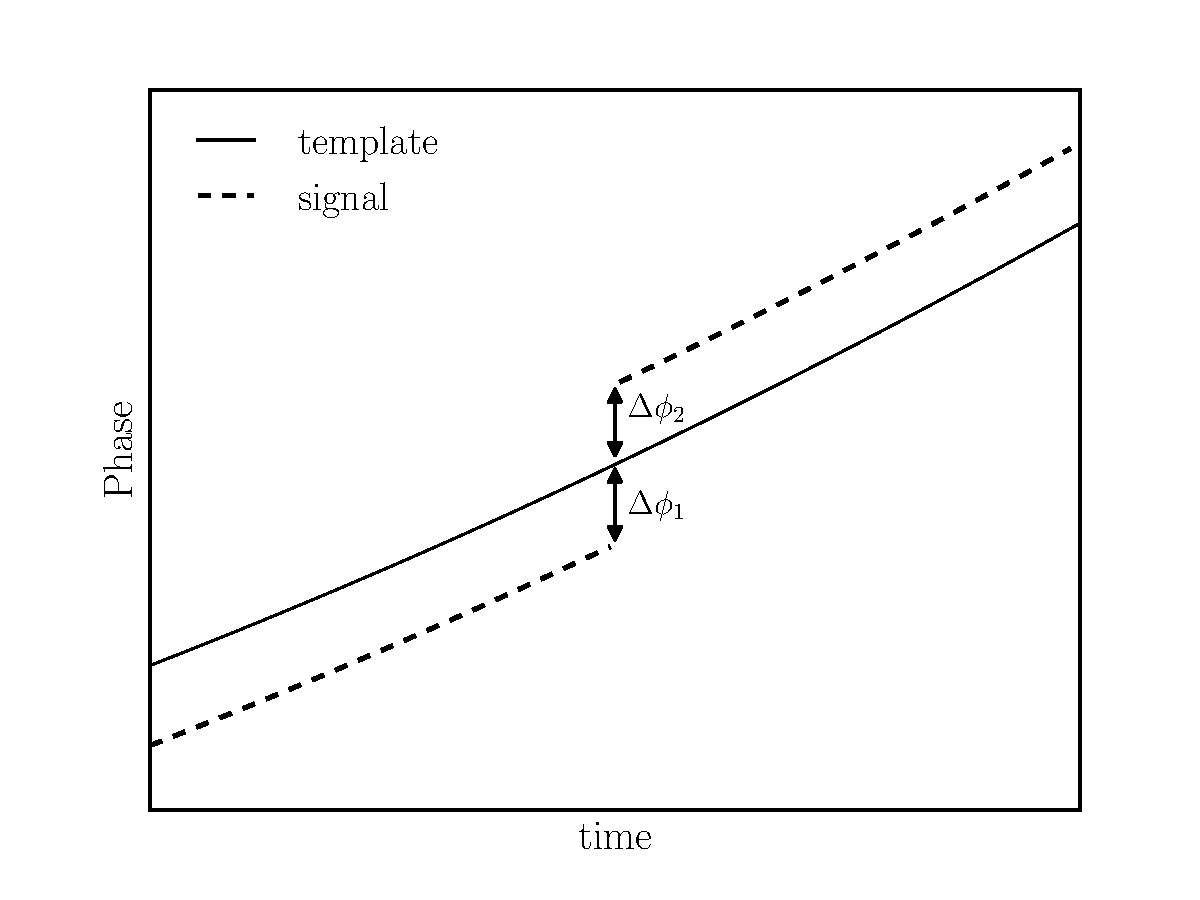
\includegraphics[width=.5\textwidth]{PhaseJump}
    \caption{Illustration of the signal and template defined in equation 
        \eqref{eqn: phase offset}}
    \label{fig: PhaseJump}
\end{figure}

To compute the matched filtering amplitude given in equation~\eqref{eqn: matched
filtering amplitude}, we factorise the integral using the additivity of
integration on intervals. This is possible only if the time dependence of the
parameter offset is discreet. 
\begin{eqnarray}
X & = &\frac{1}{T }\left(\int_{0}^{T /2}e^{i\Delta\phi_{1}} dt  + 
\int_{T/2}^{T} e^{i\Delta\phi_{2}}dt\right)\\
& = & \frac{1}{2}\left(e^{i\Delta\phi_{1}} + e^{i\Delta\phi_{2}}\right).
\end{eqnarray}
The absolute square value of the matched filtering amplitude is then
\begin{eqnarray}
|X|^{2}& = &\frac{1}{4}\left(e^{i\Delta\phi_{1}} + e^{i\Delta\phi_{2}}\right) \left(e^{-i\Delta\phi_{1}} + e^{-i\Delta\phi_{2}}\right)\\
& = &\frac{1}{4} \left(2 + e^{i(\Delta\phi_{1} - \Delta \phi_{2})} +  e^{-i(\Delta\phi_{1} - \Delta_{\phi_{2}})} \right) \\
& = &\frac{1}{2}\left(1 + \cos(\Delta\phi_{1} - \Delta\phi_{2})\right).
\end{eqnarray}
The mismatch can then be calculated from Eqn.~\eqref{eqn: full mismatch}.
\begin{equation}
m = \frac{1}{2}\left(1 - \cos(\Delta\phi_{1} - \Delta\phi_{2})\right).
\label{eqn: two subdomain phase mismatch}
\end{equation}
From this result we that it is not the phase difference with respect to the
Taylor expansion which is important, but the phase jump between the two
subdomains. For $\Delta \phi_{1} = \Delta \phi_{2}$ the mismatch vanishes
demonstrating that this method is consistent with a single subdomain model where
the phase offset does not produce a mismatch.


\paragraph{Comparing with a signal injection} We can verify equation
\eqref{eqn: two subdomain phase mismatch} by comparing with the results of a
signal injection. This involves defining the signal such that it describes two
subdomains with a phase offset, then injecting and recovering the signal using
\texttt{LALApps} software. We do this in the absence of noise and compute the mismatch 
against a perfectly matched signal.  The signal comprises two adjacent
transient windows of fixed duration. We set the phase offset in the first subdomain
to zero and subject the second subdomain to a phase
jump $\Delta \phi$, therefore 
\begin{align}
    \Delta \phi_{1} &= 0 &  \textrm{ and } && \Delta \phi_{2} =& \Delta\phi.
\end{align}
Increasing $\Delta\phi$ and measuring the mismatch the results along
with the prediction of equation~\eqref{eqn: two subdomain phase mismatch} are
plotted in figure~\ref{fig: two plot}
\begin{figure}
\centering
\includegraphics[width=0.65\textwidth]{Exact_analytic_phase_two_subdomains}
\caption{Plot of the theoretical prediction of equation~\eqref{eqn: two subdomain
phase mismatch} given a time dependent phase offset as in equation\eqref{eqn:
phase offset}. This is compared  with a signal injection and recovery
using \texttt{LALapps} software.}
\label{fig: two plot}
\end{figure}•

\FloatBarrier
\subsection{Generalisation to N-subdomains}
Take now a signal over observation time $T$ cut into $N$ equal length subdomains
each of which suffers a phase offset $\Delta \phi_{i}$ with respect to the same
reference time. Then the matched filtering amplitude can be written
\begin{eqnarray}
X & = & \frac{1}{T}\left(\int_{0}^{t_{1}}e^{i\Delta\phi_{1}} dt + 
\int_{t_{1}}^{t_{2}}e^{i\Delta\phi_{2}} dt + \dots + 
\int_{t_{N-1}}^{t_{N}}e^{i\Delta\phi_{N}} dt \right) \\
& = &  \frac{1}{T}\left(\frac{T}{N}e^{i\Delta\phi_{1}} + 
\frac{T}{N}e^{i\Delta\phi_{2}} + \dots + \frac{T}{N}e^{i\Delta\phi_{n}} \right)\\
& = & \frac{1}{N} \sum_{i=1}^{N}e^{i\Delta \phi_{i}}.
\end{eqnarray}
Squaring the matched filtering amplitude and simplifying
\begin{eqnarray}
|X|^{2} & = &  \frac{1}{N^{2}} \left(\sum_{i=1}^{N}e^{i\Delta \phi_{i}}\right)\left(\sum_{j=1}^{N}e^{-i\Delta \phi_{j}}\right) \\
|X|^{2} & = &  \frac{1}{N^{2}} \sum_{i=1}^{N}e^{i\Delta \phi_{i}}\left(\sum_{j=1}^{N}e^{-i\Delta \phi_{j}}\right) \\
& = & \frac{1}{N^{2}} \sum_{i=1}^{N}e^{i\Delta \phi_{i}}\left(e^{-i\Delta \phi_{i}} +  \sum_{\substack{j=1 \\j\ne i}}^{N}e^{-i\Delta \phi_{j}}\right) \\
& = & \frac{1}{N^{2}} \left(\sum_{i=1}^{N}1 +   \sum_{i=1}^{N}\sum_{\substack{j=1 \\j\ne i}}^{N}e^{i(\Delta\phi_{i}-\Delta \phi_{j})}\right) \\
& = & \frac{1}{N^{2}} \left(N +   \sum_{i=1}^{N}\sum_{\substack{j=1 \\j\ne i}}^{N}\cos(\Delta\phi_{i} - \Delta\phi_{j}) + i\sin(\Delta\phi_{i} - \Delta\phi_{j})\right).
\end{eqnarray}
In this final summation for each pair $(i,j)$ the corresponding pair $(j, i)$
will exist in the sum. This leads to a cancellation of the imaginary part and a
doubling of the real part
\begin{equation}
|X|^{2}  = \left(\frac{1}{N} + \frac{1}{N^{2}}\sum_{i=1}^{N}\sum_{\substack{j=1 \\j\ne i}}^{N} \cos(\Delta\phi_{i} - \Delta \phi_{j})\right).
\end{equation}•
Then the mismatch is given by:
\begin{equation}
m = 1 - \frac{1}{N} - \frac{1}{N^{2}}\sum_{i=1}^{N}\sum_{\substack{j=1 \\j\ne i}}^{N} \cos(\Delta\phi_{i} - \Delta\phi_{j}).
\label{eqn: phase mismatch}
\end{equation}•
